\documentclass[12pt]{article}

\usepackage{cite}
\usepackage[colorlinks,
linkcolor=blue,
anchorcolor=black,
citecolor=black]{hyperref}
\usepackage{graphicx} 
\usepackage{float}
\usepackage{subfigure}
\usepackage{geometry}
\geometry{a4paper,scale=0.82}


\author{Yanlong Sun}
\title{Brain Segmentation Using U-Net}
\begin{document}
\maketitle

\begin{abstract}
MRI can provide important information for surgeon before the surgery and provide researchers with more immediate information to study the organ structure. However, manually extracting is always costly. This experiment utilized a deep learning model to segment the brain automatically and achieved a great performance.
\end{abstract}


\section{Introduction}
In this experiment, we replicated a deep learning model with the U-Net architecture \cite{buda} to segment the brain MRI. After simply amended the input and output, we can easily utilize this model to segment brain MRI in different size with a high accuracy.


\section{Method}

\subsection{Preprocessing}
The image data we used in this experiment is Calgary-Campinas-359 \cite{dataset}(CC-359) dataset, which contains the brain MRI and the corresponding brain mask of 359 patients. However, images varied significantly between patients in terms of size, for instance, the aspect ratio of some images in this dataset are about 1:2 but others are 2:1. In order to make these image data have the same size to be segmented by the fully convolutional neural network. We need to preprocess the image data by the following steps:
\begin{itemize}
	\item Use 'load\_nii' function in MATLAB to obtain slices and masks from the '.nii.gz' file.
	\item Pad zeros to the slices and masks at the same time according to their aspect ratio.
	\item Center crop the slices and masks into size of 256*256.
\end{itemize} 


\subsection{Segmentation}
We kept the structure of the original model but used different dataset to train the neural network. After training on CC0001-CC0030
of CC-359, about 5000 slices, we got the Average Dice coefficient of 98.36\% on 7 groups of slices, as shown in Figure 1. Examples of segmentations with ground truth masks presented in Figure 2.
\begin{figure}[H] 
\centering 
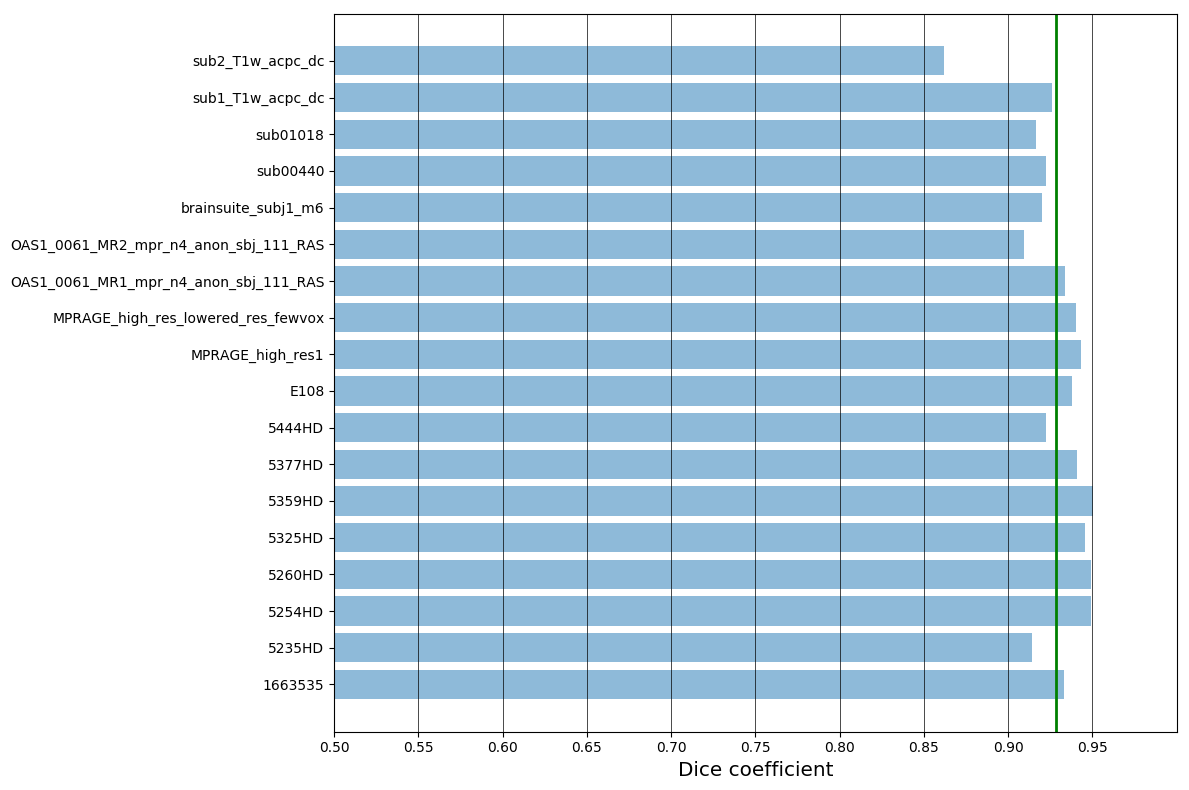
\includegraphics[width=0.8\textwidth]{DSC} 
\caption{Dice Coefficient of Test data} 
\label{DSC} 
\end{figure}

\begin{figure}[H]
\centering 
\subfigure{
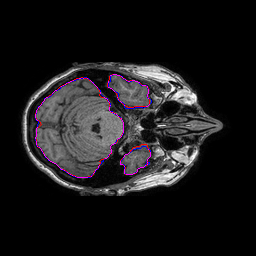
\includegraphics[width=0.3\textwidth]{CC0031}}
\subfigure{
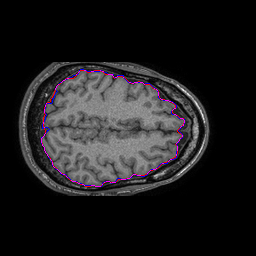
\includegraphics[width=0.3\textwidth]{CC0032}}
\subfigure{
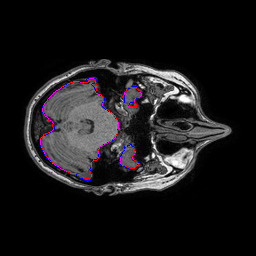
\includegraphics[width=0.3\textwidth]{CC0034}}
\caption{Examples of segmentation}
\end{figure}



\subsection{Postprocessing}
After predicting by the trained model, we got the prediction information in the 'mat' format. Then, we added these slices and predicted masks up respectively and convert them back to '.nii.gz' file.

\section{Conclusion}
In conclusion, we replicated this deep learning model and make it easier to execute even the image data are in significantly various sizes, apart from that, we also converted the prediction results into the common format, which is convenient for researchers to analyse.




\bibliography{reference}
\bibliographystyle{plain}

\end{document}